\documentclass[twocol]{ametsocV6.1}
\usepackage[a4paper, total={17cm, 25cm}, left=2cm, top=3cm]{geometry}
\usepackage{hyperref}
\usepackage[separate-uncertainty=true]{siunitx}
\usepackage{csvsimple}
\usepackage{cprotect}
\usepackage{comment}
\usepackage{tabularx}
\usepackage{makecell}
\usepackage{float}

\DeclareSIUnit\clight{\text{\ensuremath{c}}}
\renewcommand{\sectionautorefname}{\S}
\renewcommand{\subsectionautorefname}{\S}
\renewcommand{\subsubsectionautorefname}{\S}
\renewcommand*{\thesubsection}{\thesection \alph{subsection}}

\renewcommand{\hmmax}{0}
\renewcommand{\bmmax}{0}

\let\subsectionautorefname\sectionautorefname

\title{
	Experimental characterisation of a superconducting quantum
	interference device
}

\authors{
	Thomas Schanzer \aff{a}
	\correspondingauthor{
		Thomas Schanzer,
		\\ \href{mailto:t.schanzer@student.unsw.edu.au}%
			{t.schanzer@student.unsw.edu.au} \\
		Word count: 2107
	}
}

\affiliation{\aff{a}{
	School of Physics, University of New South Wales,
	Sydney, Australia
}}

\abstract{
	We present measurements of the key properties of a superconducting
	quantum interference device (SQUID), including the critical current
	threshold
	for superconductivity, the periodic oscillations in the voltage across the
	device with changing magnetic field and discrete Shapiro steps
	in voltage when a microwave-frequency electric field is applied.
	We establish rigorous techniques for analysing the relevant data that
	may be applied to other SQUIDs and sensitive magnetic field measurements.
}

\begin{document}
\vspace{5cm}
\maketitle

\section{Introduction} \label{sec:intro}
\subsection{Structure and key properties of the SQUID}
A superconducting quantum interference device, or SQUID, consists of
a superconducting ring, interrupted by two thin non-superconducting
regions---Josephson junctions---on opposite sides, as shown in Figure
\ref{fig:diagram}. While a full quantum mechanical description of the device
is beyond the scope of this report, we will briefly outline some of its
key properties.

\begin{figure}[ht]
	\centering
	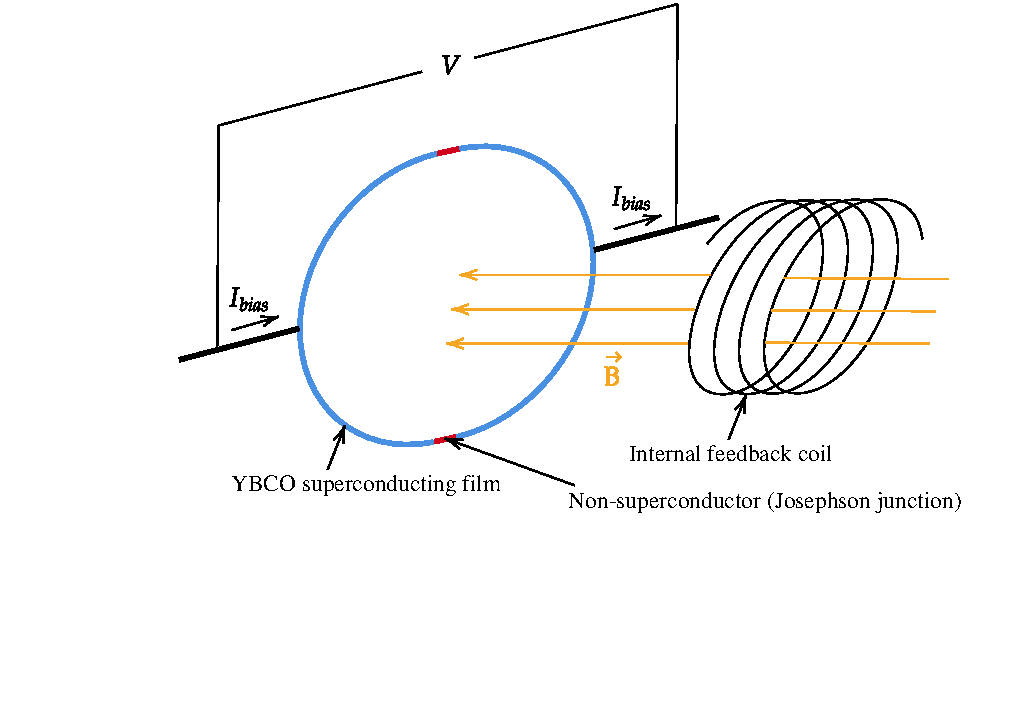
\includegraphics[width=\linewidth]{../figures/diagram.pdf}
	\caption{
		Diagram of the SQUID used in this work.
	}
	\label{fig:diagram}
\end{figure}

A biasing current may be passed between the two sides
of the coil. Below the critical
temperature of the superconductor, the Josephson junctions create a
current threshold, above which the ring will cease to superconduct
and a potential difference $V$ will develop between the two sides.
If each junction has a critical current $I_c$, the critical current of
the SQUID as a whole will be $2I_c$.

Secondly, due to the ring's superconductivity, the application of
an external magnetic field induces a screening current that circulates
in the ring to maintain zero magnetic flux through it; if the flux were to
vary, a potential difference would appear in the loop in accordance with
Faraday's law. This screening current is superimposed upon any biasing
current passing through the ring, reducing the critical current.
If the external magnetic field is increased further, the critical current may
be exceeded, destroying the superconductivity, causing a voltage
to develop across the loop and allowing some flux to enter.
It may be shown that only a flux of exactly
$\Phi_0 \equiv h/2e \approx \SI{2.07e-15}{\weber}$, known as the flux
quantum, may be allowed to enter the loop before
superconductivity is restored, the voltage across the loop returns to zero
and the process restarts. This causes the voltage to be periodic in the
applied magnetic field, and by counting the number of periods one may
determine the flux through the loop with extremely high resolution, owing to
the small value of $\Phi_0$. For this reason, SQUIDs are used to measure
magnetic fields in applications where extreme sensitivity is required.

A third property of the SQUID is that, in the presence of an oscillating
electric field, the voltage across the loop may increase in discrete steps
(\emph{Shapiro steps})
with increasing biasing current. This is a consequence of the AC Josephson
effect, the phenomenon whereby the current in a Josephson junction naturally
oscillates in time. While a rigorous explanation of this effect is well beyond
the scope of the report, we will use the known result
\begin{equation}
	\Phi_0 \equiv \frac{h}{2e} = \frac{\Delta V}{\nu} \label{eqn:h-e_ratio}
\end{equation}
to determine $\Phi_0$ given the size $\Delta V$ of the voltage steps
and the frequency $\nu$ of the oscillating electric field.

\subsection{Outline}
In \autoref{sec:methods}, we will briefly describe the experimental setup
and procedure. In \autoref{sec:results}, we will present and analyse
measurements of the SQUID's properties, beginning with its superconducting
$I$-$V$ characteristics in \autoref{sec:iv}, followed by the periodic
voltage-flux relationship in \autoref{sec:vphi} and the microwave-induced
Shapiro steps in \autoref{sec:shapiro}. In \autoref{sec:discussion} we will
discuss the limitations of our work and suggest future improvements,
before concluding the report in \autoref{sec:conclusion}.



\section{Methods} \label{sec:methods}
The particular device tested in this work is the Star Cryoelectronics
\emph{Mr SQUID}, which uses a Y$_1$Ba$_2$Cu$_3$O$_7$ high-temperature
superconducting film ($T_c \approx \SI{90}{\kelvin}$). The reader is referred
to the \emph{Mr SQUID User's Guide} \citep{squid_guide} for a detailed
description.

The device was immersed in liquid nitrogen at $\SI{77}{\kelvin}$. The biasing
current and magnetic field were varied by a control unit supplied by
the device's manufacturer, with the current through and voltage across the
device being measured and digitised by internal analog-to-digital converters
before being sent to a computer for analysis. The oscillating electric
field needed to create the Shapiro steps in \autoref{sec:shapiro} was created
by a signal generator connected to an antenna inside the dewar.

In \autoref{sec:iv} and \autoref{sec:shapiro}, the SQUID control unit was set
to supply a triangle-wave biasing current and measure the resulting voltage,
showing the relationship between the current
and voltage in the device. In \autoref{sec:vphi}, the triangle-wave
current was instead supplied to an internal coil in the SQUID, generating a
proportional magnetic field and showing the relationship between voltage and
flux.

\section{Results} \label{sec:results}
\subsection{$I$-$V$ characteristics} \label{sec:iv}
Figure \ref{fig:iv}a shows the relationship between the biasing current and voltage across the SQUID. A clear
superconducting region, where voltage is independent of current,
is visible. Beyond some critical current, the superconductivity ceases and
voltage varies approximately linearly with current.

\begin{figure}[ht]
	\centering
	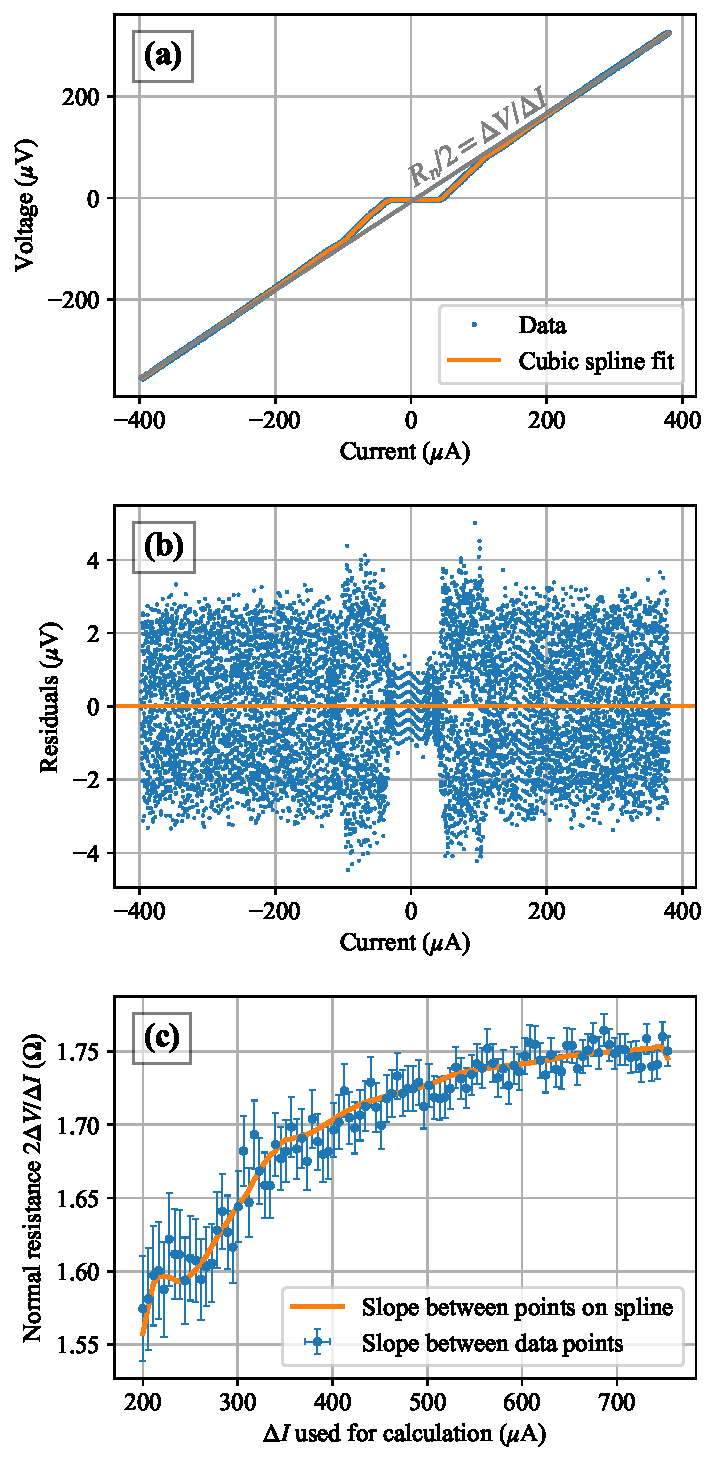
\includegraphics[width=\linewidth]{../figures/iv.pdf}
	\caption{
		\textbf{(a)}: $I$-$V$ curve of the SQUID, with a cubic smoothing spline
		shown in orange. Current and voltage uncertainties for all data points
		were estimated to be $\SI{1}{\micro\ampere}$ and $\SI{1}{\micro\volt}$
		respectively.
		\textbf{(b)}: Residuals of the cubic spline fit. The non-uniformity
		of their magnitude is due to a contribution from the current
		uncertainty, which is larger in the upward-sloping regions.
		\textbf{(c)}: The normal resistance computed from the $I$-$V$ curve
		as a function of the horizontal separation of the points used.
	}
	\label{fig:iv}
\end{figure}

The \emph{normal resistance} of the device is the value of its resistance
when the superconducting region is ignored, and is measured by finding the
gradient between the endpoints of the $I$-$V$ curve and doubling the result
(because there are two Josephson junctions in parallel),
as indicated by the grey line in Figure \ref{fig:iv}a.
Since the curve is obviously nonlinear, the measured value can depend on the
extent of the curve that is measured; one naturally asks what the
horizontal distance between the endpoints should be.
In Figure \ref{fig:iv}c, we show the
slope between pairs of points (symmetric about the centre of the $I$-$V$ curve)
as a function of their horizontal separation $\Delta I$ and observe that
the result converges to a fixed value, which we take to be the correct one.
To reduce the effect of noise on the result, we use a cubic spline fit to the
curve (the residuals of which are shown in Figure \ref{fig:iv}b) when
computing slopes, and compare this to the slopes between the original data
points in order to estimate the uncertainty. Our final result is
\begin{equation}
	R_n = \SI{1.75 \pm 0.01}{\ohm},
\end{equation}
which is larger than the value of $\SI{1.6}{\ohm}$ measured by the
manufacturer, possibly due to degradation of the device over several years
of repeated cooling and warming.

In order to find the critical current at which superconductivity ceases,
we model the transitions between the superconducting and normal regions
of the $I$-$V$ curve using hyperbolae of the form
\begin{equation}
	(y - m_1 x - b_1)(y - m_2 x - b_2) = c. \label{eqn:hyperbola}
\end{equation}
One asymptote, $y = m_1 x + b_1$, slopes upwards to match the normal region,
while the other, $y = m_2 x + b_2$, is horizontal, matching the superconducting
region. The constant $c$ determines the sharpness of the transition. Using
orthogonal distance regression to fit (\ref{eqn:hyperbola}) to the two
bends, the critical current may then be determined from the point of
intersection of the asymptotes. Figure \ref{fig:knee_fits} shows the results
of this procedure; the hyperbola happens to be an excellent model, fitting
the data with a coefficient of determination exceeding $0.99$.
Averaging the values from the left and right knees,
we find that the critical current of the SQUID is
\begin{equation}
	2 I_c = \SI{39.1 \pm 1.2}{\micro\ampere}. \label{eqn:critical_current}
\end{equation}
This deviates significantly from the value of \SI{68}{\micro\ampere}
measured by the manufacturer approximately five years prior to our
work; we also attribute this to degradation of the device over time.

\begin{figure*}[ht]
	\centering%
	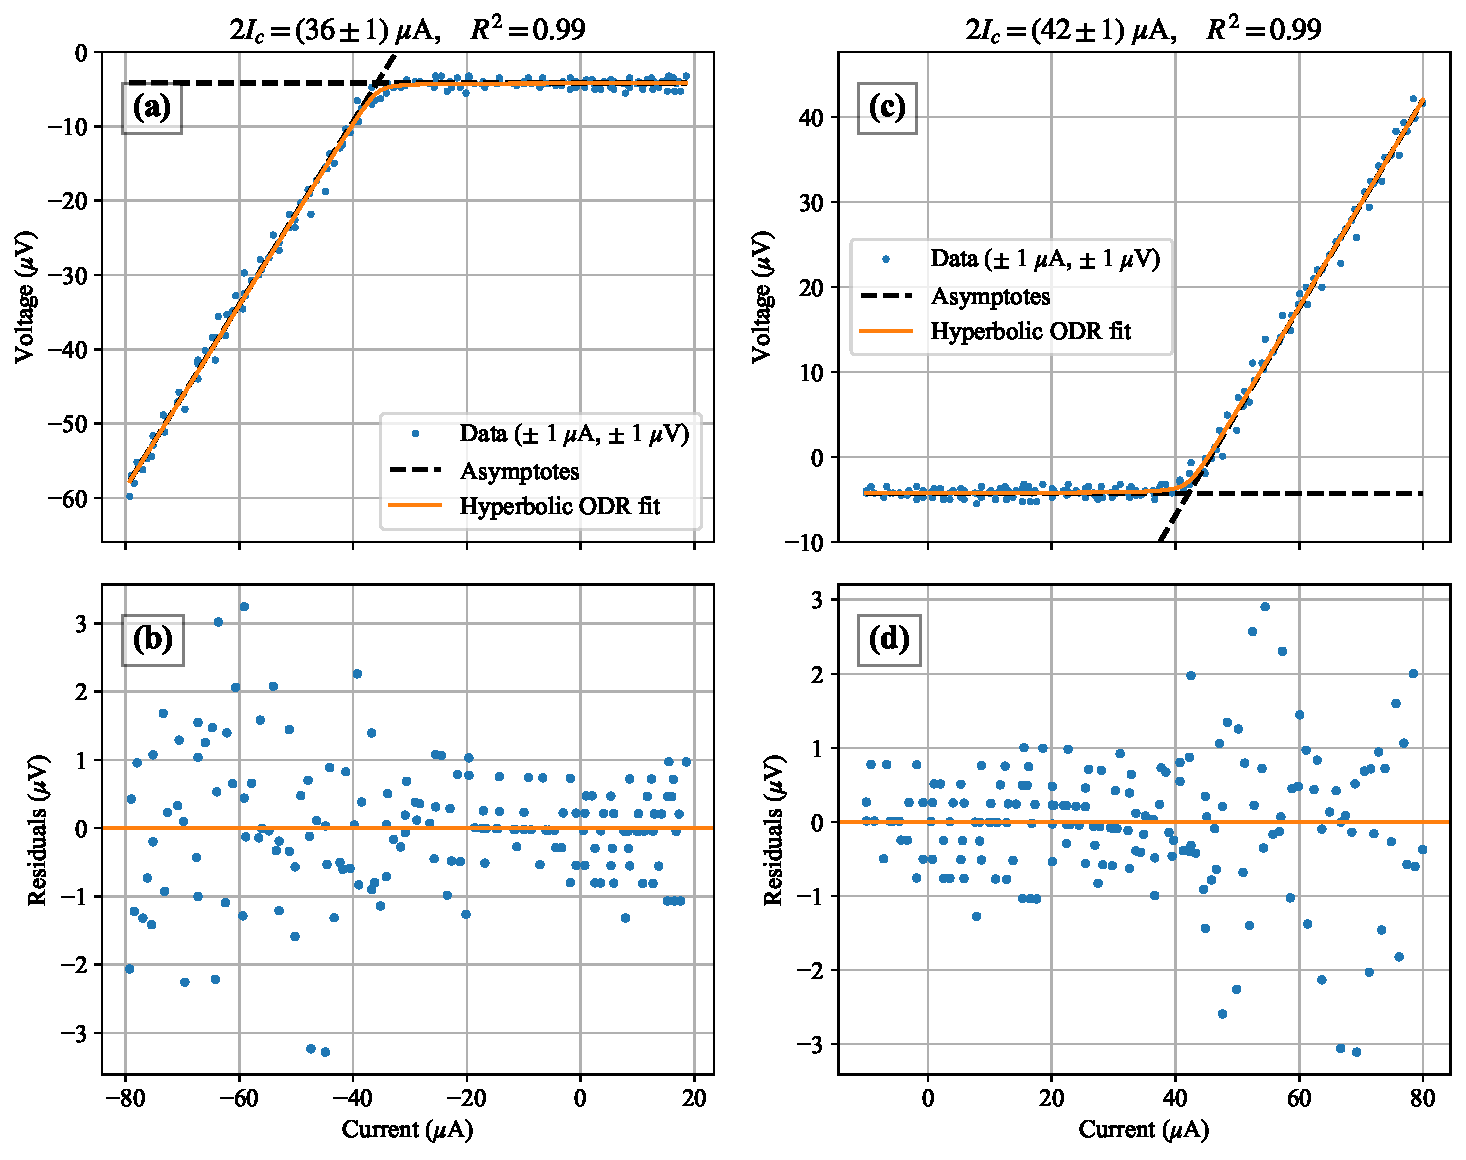
\includegraphics[width=\linewidth]{../figures/knee_fits.pdf}
	\caption{
		\textbf{(a)}, \textbf{(c)}: hyperbolic fits to the bends in
		the $I$-$V$ curve (orange), with asymptotes indicated by dashed
		black lines. The critical current $2I_c$ is the horizontal position
		of the intersection of the asymptotes. Error bars are omitted for
		clarity; the uncertainties in the $x$ and $y$ values are
		$\SI{1}{\micro}{\ampere}$ and $\SI{1}{\micro\volt}$ respectively.
		\textbf{(b)}, \textbf{(d)}: residuals of the orange fits.
	}
	\label{fig:knee_fits}
\end{figure*}

It was also possible to apply a constant magnetic field to the SQUID during
the $I$-$V$ sweeps by passing a current through the internal feedback coil.
The results shown in Figure \ref{fig:knee_fits} are for a coil current
of $\SI{40}{\micro\ampere}$, which appeared to produce the sharpest
transitions between the superconducting and normal regions.
As an extension, $I$-$V$ curves were acquired for a range of
coil currents, allowing the measurement of critical current as a function of
applied field. The result is shown in Figure \ref{fig:Ic_vs_flux};
the critical current periodic in the applied field as anticipated
in \autoref{sec:intro}. It also appears that setting the applied field
so that the bends in the $I$-$V$ curve are \emph{less} sharp results in
a higher critical current (at least according to the standard definition).

\begin{figure}[ht]
	\centering
	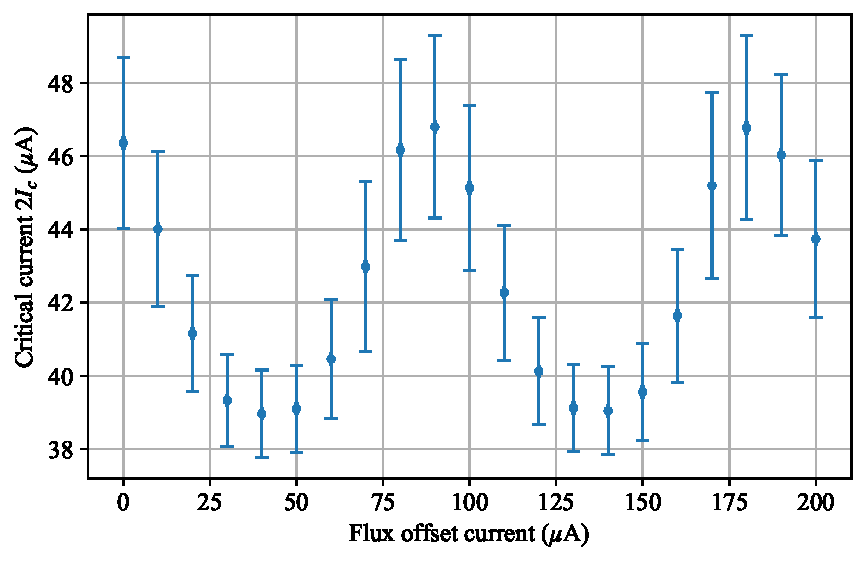
\includegraphics[width=\linewidth]{../figures/Ic_vs_flux.pdf}
	\caption{
		Plot of critical current as a function of the current passed
		through the internal feedback coil, which is proportional to
		the applied magnetic field.
	}
	\label{fig:Ic_vs_flux}
\end{figure}

\subsection{$V$-$\Phi$ characteristics} \label{sec:vphi}
\begin{figure*}[ht]
	\centering
	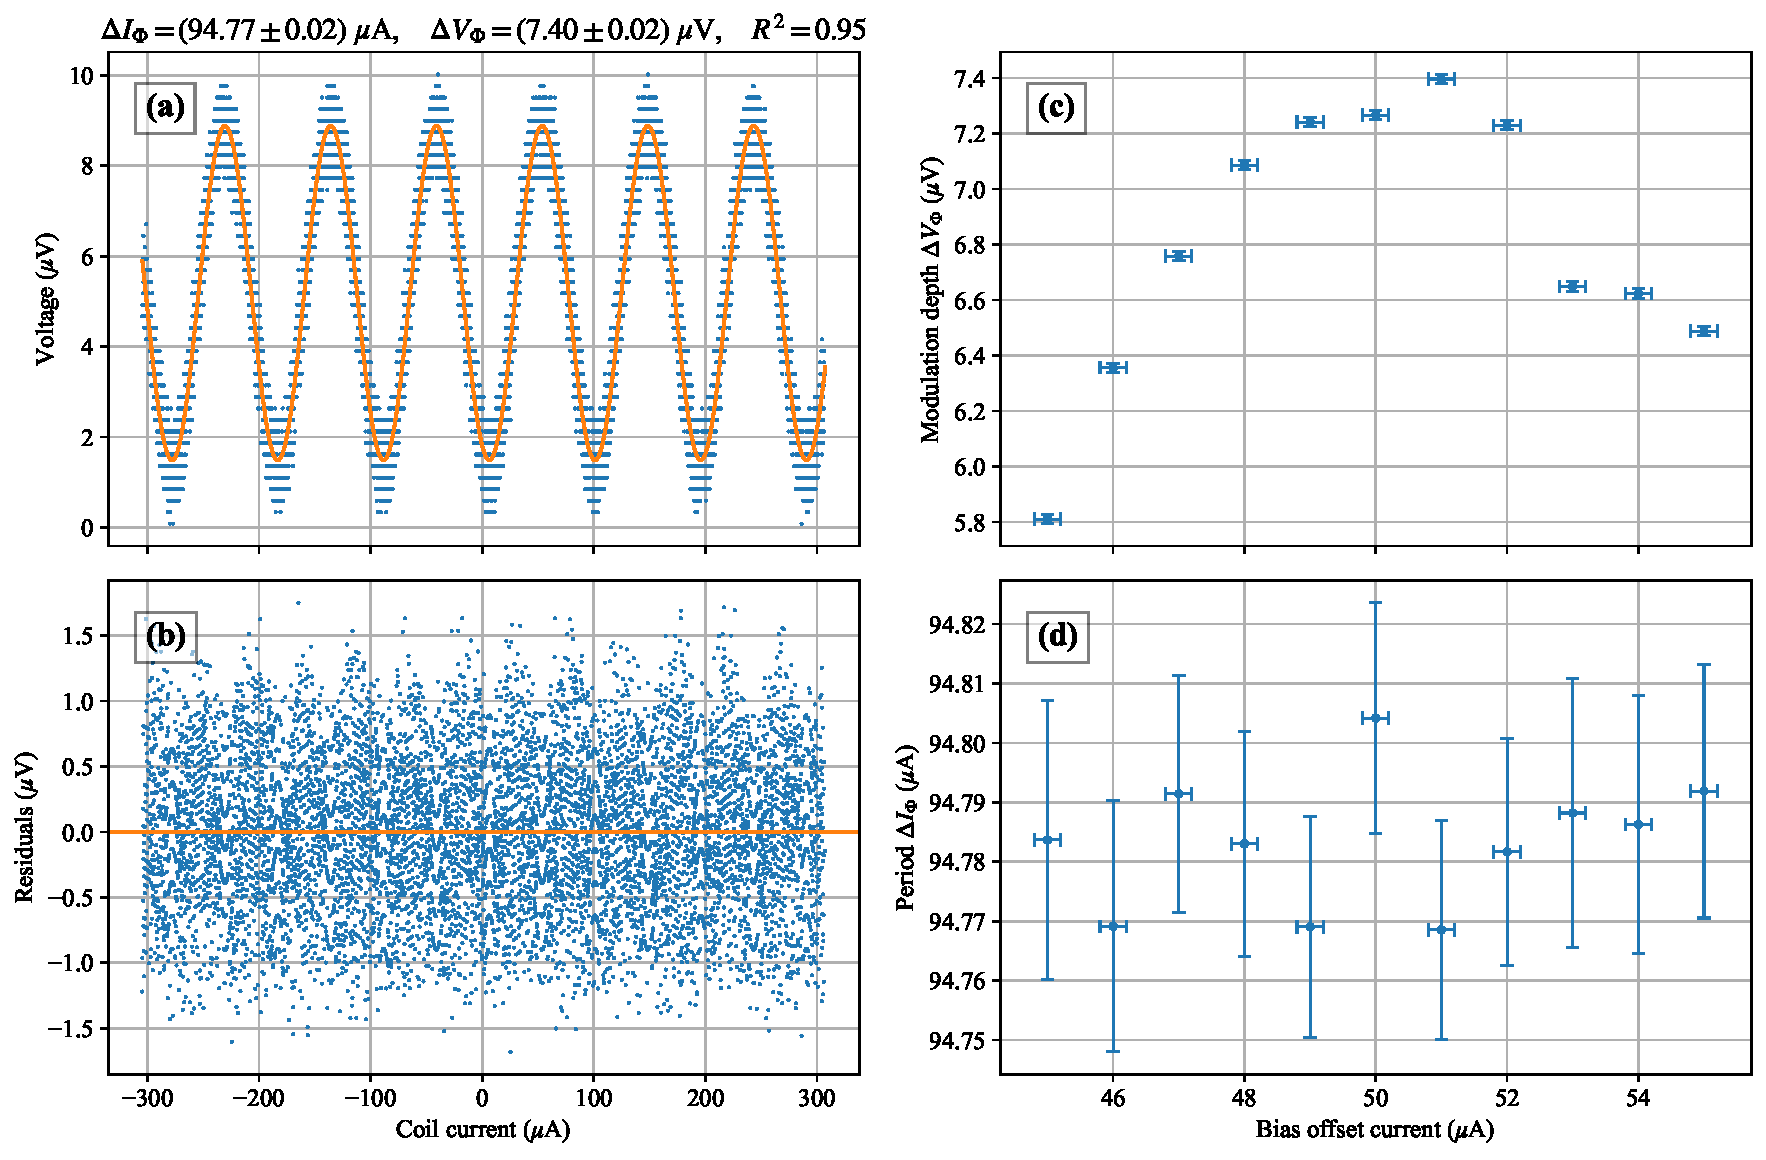
\includegraphics[width=\linewidth]{../figures/vphi.pdf}
	\caption{
		\textbf{(a)}: Voltage across the SQUID as a function of the current through the
		internal feedback coil, which is proportional to the applied magnetic
		field. Error bars are omitted for clarity;
		current and voltage uncertainties for all data points
		were estimated to be $\SI{1}{\micro\ampere}$ and $\SI{1}{\micro\volt}$
		respectively. A sinusoidal ODR fit is shown in orange.
		\textbf{(b)}: Residuals of the sinusoidal fit in (a).
		\textbf{(c), (d)}: Plots of the peak-to-peak voltage amplitude
		and period, respectively, as functions
		of the bias current passing across the SQUID.
	}
	\label{fig:vphi}
\end{figure*}

Figure \ref{fig:vphi} shows the periodic variation of the voltage across
the SQUID as the applied magnetic field (controlled by the current through
an internal coil) is changed. By fitting a sinusoidal curve to the data using
orthogonal distance regression, the peak-to-peak amplitude
$\Delta V_\Phi$ and period $\Delta I_\Phi$ were determined.

The biasing current was set close to
the critical current of the SQUID to ensure that changes in flux caused
the induced current in the superconducting loop to momentarily exceed the
critical current and allow a flux quantum to enter. It was observed that
$\Delta V_\Phi$ depended sensitively on the biasing current, while
$\Delta I_\Phi$ was constant, as shown in Figure \ref{fig:vphi}c,d.

Unfortunately, the measured $\Delta V_\Phi$ was at most
$\SI{7.4 \pm 0.02}{\micro\volt}$, inconsistent with the manufacturer's value of
$\SI{8.9}{\micro\volt}$. $\Delta I_\Phi$, measured to be
$\SI{94.78 \pm 0.01}{\micro\ampere}$, was also inconsistent with the
manufacturer's value of $\SI{97.5}{\micro\ampere}$. Both of these discrepancies
could also be due to degradation of the device over time.


\subsection{Shapiro steps} \label{sec:shapiro}
Figure \ref{fig:shapiro_steps}a shows the $I$-$V$ curve of the SQUID
in the presence of an external microwave-frequency electric field supplied
by a signal generator. Three discrete steps in the voltage are observed
as the biasing current is increased.

In order to determine $\Phi_0$, we must determine the vertical
separation $\Delta V$ between the steps, which in turn requires us to
determine the positions of the steps. Recognising that the steps are the
positions of minimum $\mathrm{d}V/\mathrm{d}I$, we fit a cubic spline
to the $I$-$V$ data and locate the minima in its derivative (the spline is
used to reduce the noise in the data, which would be amplified by
differentiation). Figure \ref{fig:shapiro_steps} shows three clear minima
in the derivative as expected; we take the uncertainties in the positions
to be the widths of the troughs at 10\% of their depths. Mapped back
onto the $I$-$V$ curve, we obtain the step positions and uncertainties
shown in Figures \ref{fig:shapiro_steps}d,e,f, which appear very reasonable.

\begin{figure*}[ht]
	\centering%
	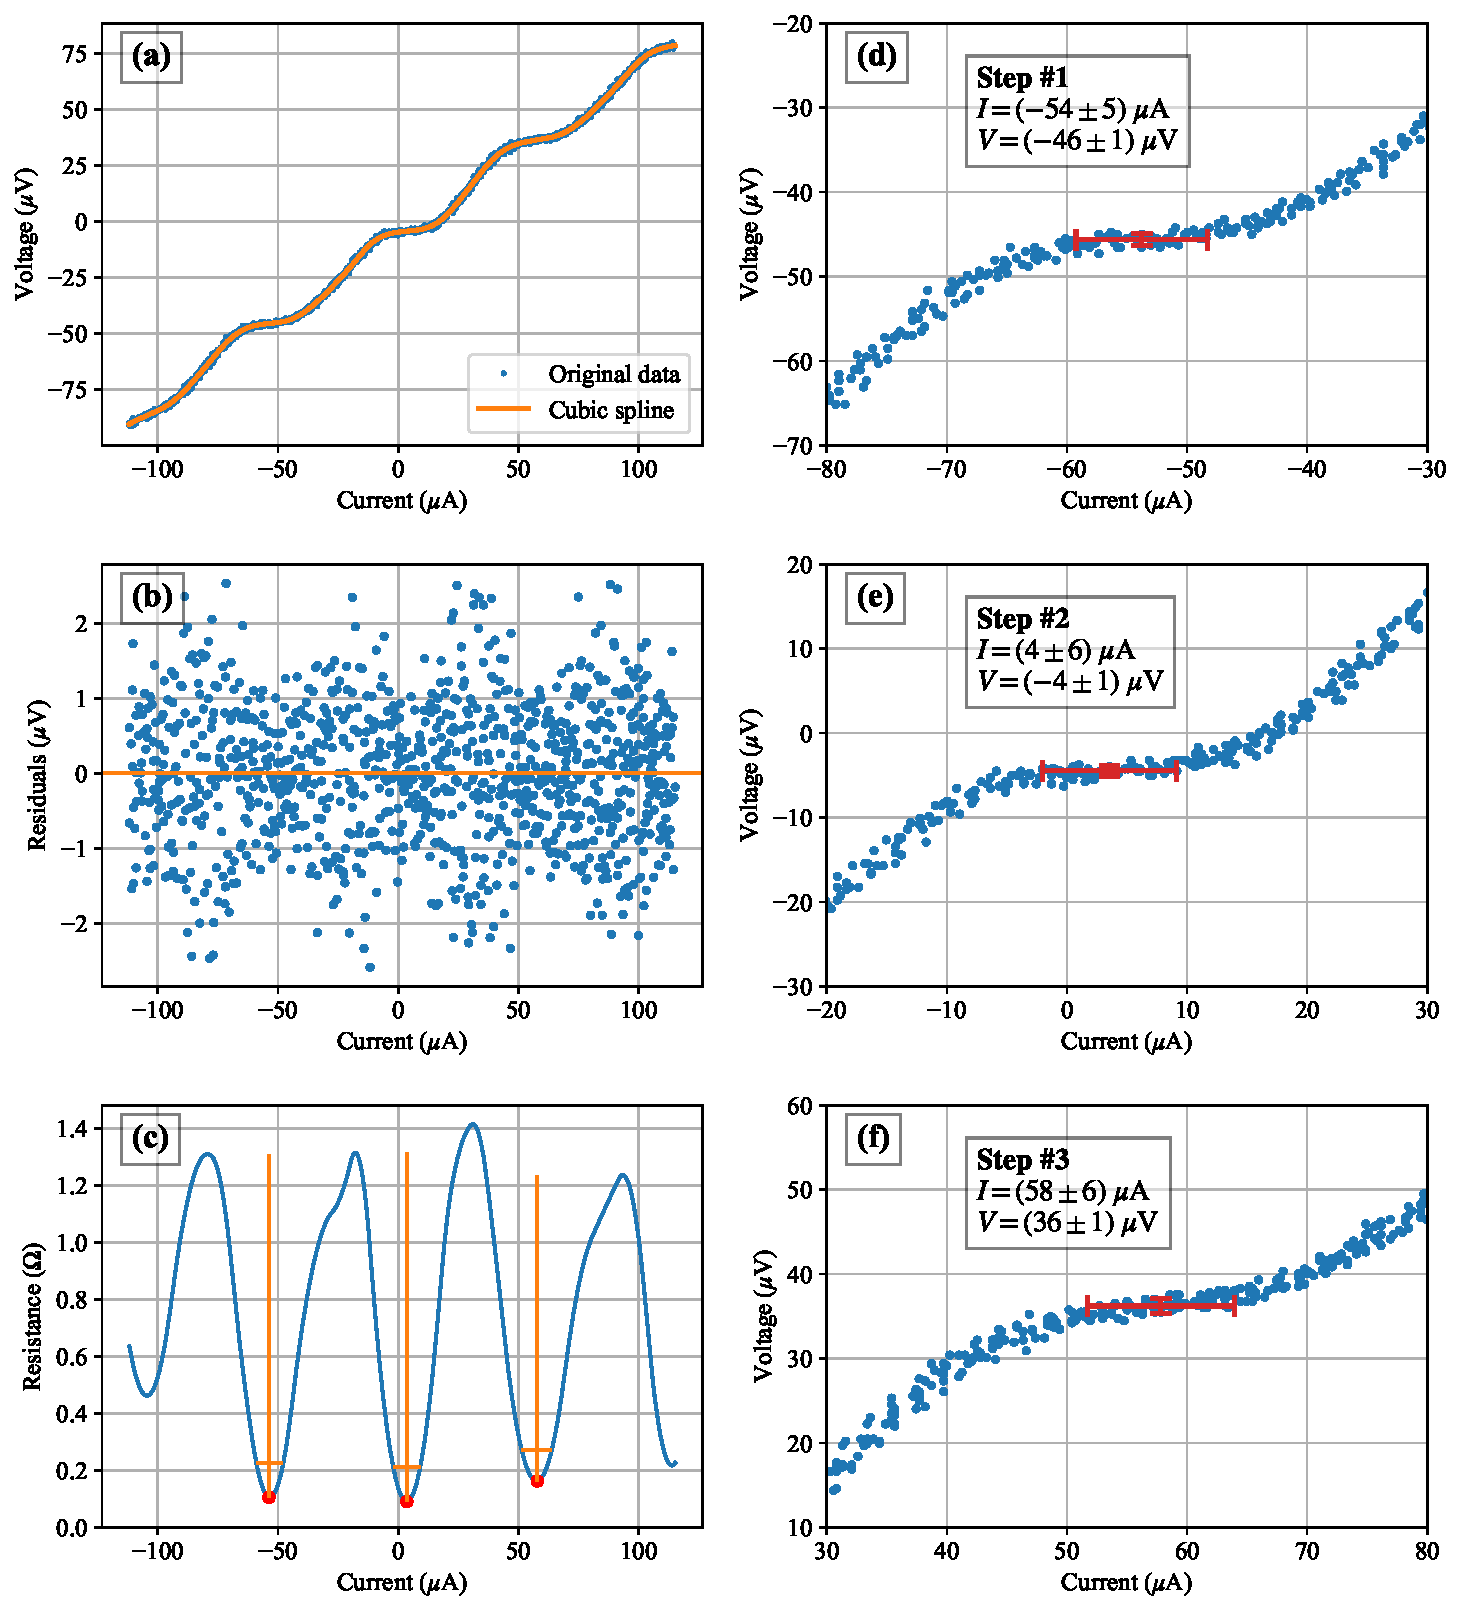
\includegraphics[width=\linewidth]{../figures/shapiro_steps.pdf}
	\caption{
		\textbf{(a)}: the $I$-$V$ curve of the SQUID when a
		$\SI{19.935}{\giga\hertz}$ oscillating electric field is applied,
		producing three Shapiro steps. Current and voltage uncertainties for
		all data points
		were estimated to be $\SI{1}{\micro\ampere}$ and $\SI{1}{\micro\volt}$
		respectively. A cubic spline fit is shown in orange.
		\textbf{(b)}: residuals of the cubic spline fit.
		\textbf{(c)}: the derivative of the cubic spline (blue curve),
		with three minima corresponding to the flat parts of the Shapiro steps.
		Vertical orange lines indicate the centres of the troughs,
		and the horizontal orange lines their widths at 10\% of the trough
		depth.
		\textbf{(d)}, \textbf{(e)}, \textbf{(f)}: enlarged views of the
		three Shapiro steps, with the calculated positions of their centres
		indicated by red error bars.
	}
	\label{fig:shapiro_steps}
\end{figure*}

Finally, substitution of the positions into (\ref{eqn:h-e_ratio}),
given the microwave frequency $\SI{19.935}{\giga\hertz}$, yields
\begin{equation}
	\Phi_0 = \frac{h}{2e} = \SI{2.05 \pm 0.04 e-15}{\weber},
\end{equation}
consistent with the accepted value of $\SI{2.068e-15}{\weber}$.

As an extension, the above procedure was repeated using $I$-$V$ curves
obtained at a range of microwave frequencies. Figure \ref{fig:step_vs_freq}
shows a plot of the step size $\Delta V$ as a function of the frequency $\nu$,
producing a straight line whose slope should be equal to $\Phi_0$. Since
the uncertainty in frequency is negligible, ordinary least squares regression
was used to fit a line to the points, yielding a slope
\begin{equation}
	\Phi_0 = \SI{2.07 \pm 0.08 e-15}{\weber},
\end{equation}
also consistent with the accepted value.

\begin{figure}[ht]
	\centering
	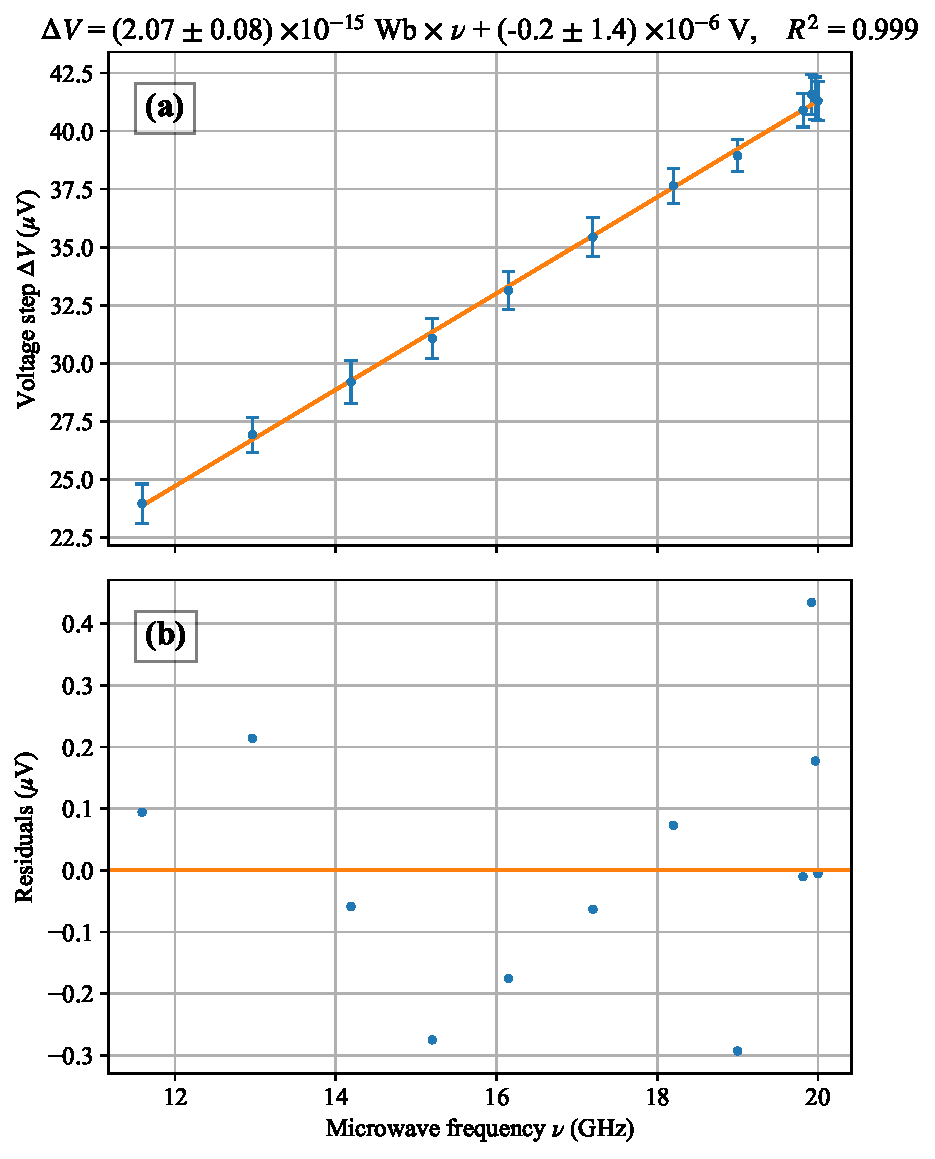
\includegraphics[width=\linewidth]{../figures/step_vs_freq.pdf}
	\caption{
		\textbf{(a)}: Plot of the Shapiro voltage step size as a function of
		microwave frequency, with a least-squares linear fit in orange.
		The equation of the line is displayed above the plot.
		The uncertainty in frequency is negligible.
		\textbf{(b)}: Residuals of the fit in (a).
	}
	\label{fig:step_vs_freq}
\end{figure}

\newpage
\section{Discussion} \label{sec:discussion}
We shall now discuss some of the factors that affected the quality of our
results. The most significant was the need to manually fine-tune the settings
on the SQUID control unit (magnetic field and biasing current offset) in
order to maximise the critical current in \autoref{sec:iv}, the
amplitude of the voltage oscillations in \autoref{sec:vphi} and the sharpness
of the Shapiro steps in \autoref{sec:shapiro}. The production of the Shapiro
steps in \autoref{sec:shapiro} also required
time-consuming fine-tuning of the microwave frequency and power. While
we have explored the dependence of our results on some of these settings
(see Figures \ref{fig:Ic_vs_flux}, \ref{fig:vphi}c-d, \ref{fig:step_vs_freq});
it appears that very small changes in the settings can significantly affect
the measured SQUID parameters. In particular, it was found that a slight
change in the position of the microwave antenna inside the dewar could
change the observed pattern of Shapiro steps. Consequently, it may be difficult to reproduce
these results reliably in future work. A possible solution would be to use
a remote-controllable measurement system that allows programmatic variation
of the settings.


\section{Conclusions} \label{sec:conclusion}
In \autoref{sec:iv} we have measured the $I$-$V$ characteristics of a SQUID,
demonstrating and measuring the critical current threshold for superconductivity
and measuring the normal resistance. The critical current was found to be a
periodic function of applied magnetic field. The device also appears to have
degraded over time, increasing the normal resistance and decreasing the
critical current.

In \autoref{sec:vphi}, we showed that the voltage across the SQUID is a
periodic function of applied magnetic field due to the quantisation of flux
through the superconducting loop. There exists a particular biasing current
that maximises the amplitude of the oscillations, but the bias current has
no effect on the period.

Finally, in \autoref{sec:shapiro}, we demonstrated that, in the presence
of an oscillating electric field, the voltage across the device increases
in discrete Shapiro steps when the biasing current is increased. By measuring
the separation of the steps for a range of frequencies, we found the value
of the magnetic flux quantum to be
$\Phi_0 = h/2e = \SI{2.07 \pm 0.08 e-15}{\weber}$, consistent with the
accepted value and with reasonable precision.

In summary, we have successfully demonstrated and measured the properties
of a SQUID. Our rigorous analysis techniques could be used to characterise
other SQUIDs and are a step towards making precise magnetic field measurements
using these sensitive devices.


\acknowledgments
The author thanks his laboratory partners J. Liang, A. Wei, T. Dunmore and
D. Dunmore for their enlightening discussion of the experiment. In particular,
he thanks J. Liang for suggesting the use of cubic spline fitting
for finding the positions of the Shapiro steps in \autoref{sec:shapiro}.

The author gratefully acknowledges the assistance of the UNSW School of Physics,
which provided the facilities and equipment for this work, and the staff
in the UNSW Higher Year Physics Laboratory, who provided guidance during
the experiment.

\datastatement
The raw data and Python code used to produce the results in this report
are available as supplementary material at
\url{https://github.com/tschanzer/SQUID}. They are also available from
the author upon request.

\bibliographystyle{ametsocV6}
\bibliography{references}

\clearpage
\appendix
\begin{center}
	Voltage and current uncertainties
\end{center}

We briefly justify our claim that the uncertainties in our voltage and
current measurements are approximately $\SI{1}{\micro\volt}$ and
$\SI{1}{\micro\ampere}$ respectively.

Figure \ref{fig:I_uncertainties} shows a plot of the triangle-wave current
supplied through either the superconducting loop or the internal feedback
coil. We fit a linear spline to it and find that the residuals of the fit
are of order $\SI{1}{\micro\ampere}$, as claimed.

\begin{figure}[ht]
	\centering
	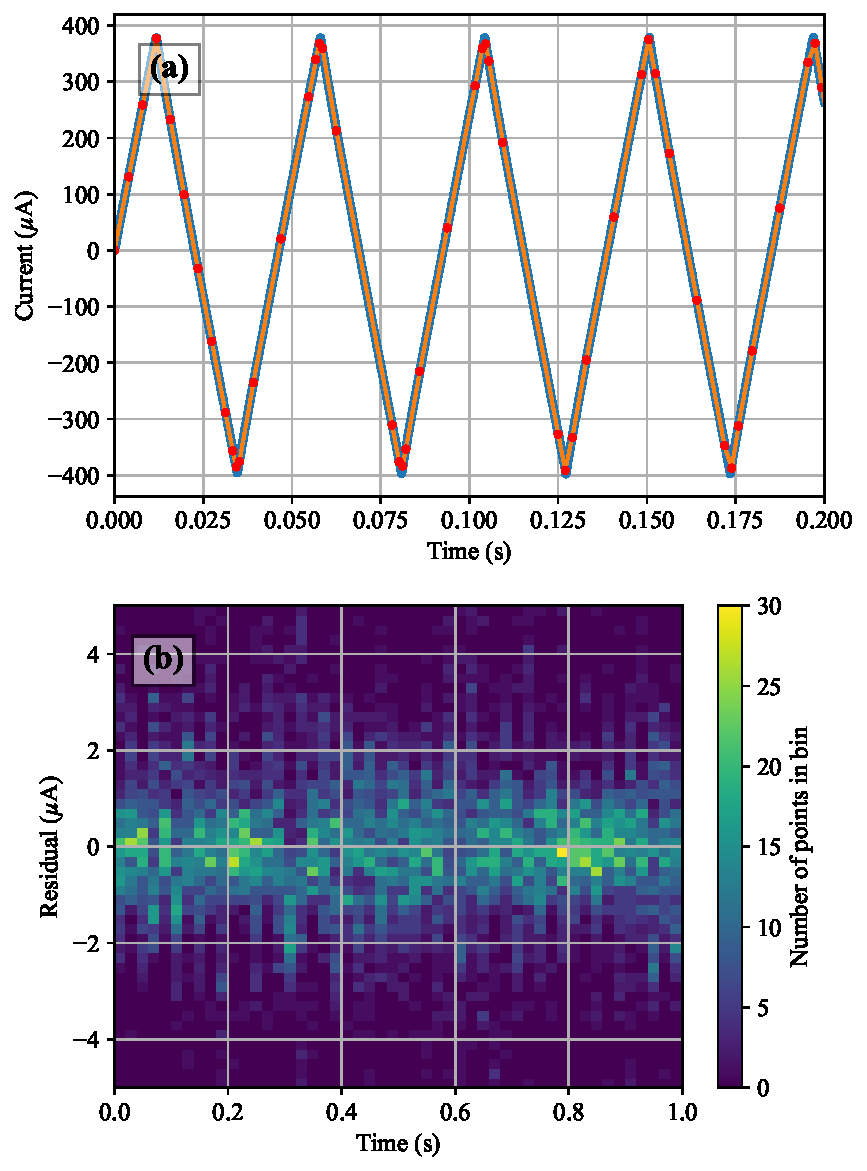
\includegraphics[width=\linewidth]{../figures/I_uncertainties.pdf}
	\caption{
		\textbf{(a)}: Plot of the measured triangle-wave current (blue),
		with linear spline fit in orange. Red points indicate the knots
		of the spline.
		\textbf{(b)}: 2D histogram of the residuals, with the colour of each
		bin indicating the number of residual data points it contains.
		The key finding is that most of the residuals are within
		$\SI{\pm 1}{\micro\ampere}$.
	}
	\label{fig:I_uncertainties}
\end{figure}

To determine the voltage uncertainty, we enlarge the superconducting potion
of the $I$-$V$ curve, where the voltage should be independent of current,
in Figure \ref{fig:V_uncertainties}. The data points in this region
deviate vertically from the mean value by up to $\SI{1}{\micro\volt}$,
justifying our claim.

\begin{figure}[ht]
	\centering
	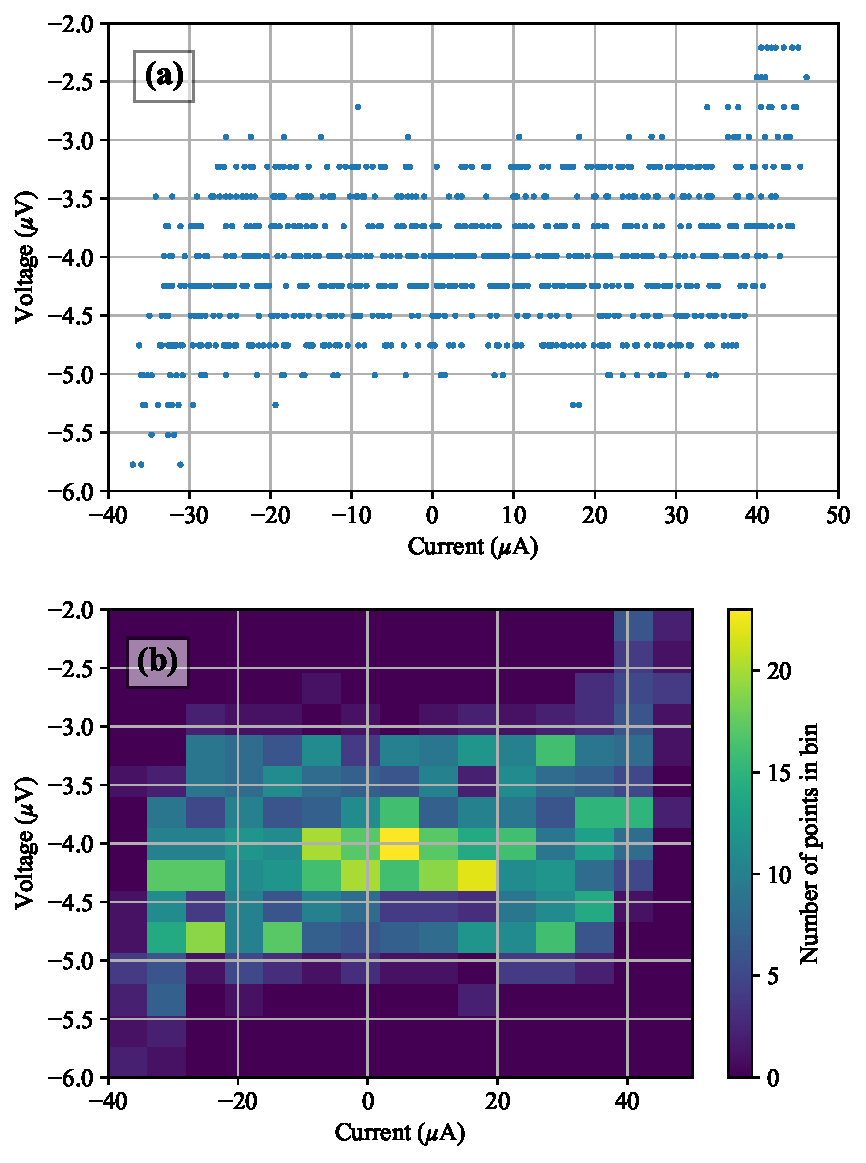
\includegraphics[width=\linewidth]{../figures/V_uncertainties.pdf}
	\caption{
		\textbf{(a)}: Enlarged view of the superconducting region of the
		$I$-$V$ curve. The appearance of several horizontal lines is due to
		the limited resolution of the analog-to-digital converter.
		Most points lie within $\SI{1}{\micro\volt}$ of the mean value at
		$\SI{-4}{\micro\volt}$.
		\textbf{(b)}: 2D histogram of the data points in (a), confirming
		the $\SI{1}{\micro\volt}$ uncertainty estimation.
	}
	\label{fig:V_uncertainties}
\end{figure}


\end{document}